\section[Review]{Review}

\subsection{Conditional Probability}

\begin{frame}{Conditional Probability}
	Bayes' theorem follows naturally from the definition of conditional probability:
	\begin{block}{Definition: Conditional Probability}
		Given two events $A$ and $B$, the conditional probability of $A \mid B$ (read \textit{A given B}) is defined as the ratio between the joint probability of $A$ \textbf{and} $B$ and the marginal probability of $B$:
		\begin{equation}
			P(A \mid B) = \displaystyle \frac{P(A \cap B)}{P(B)}
			\nonumber
		\end{equation}
	\end{block}
\end{frame}

\begin{frame}{Conditional Probability}
	When events $A$ and $B$ are independent, we can write:
	\begin{equation}
		P(A \cap B) = P(A) \, P(B)
		\text{\quad or \quad} P(A, B) = P(A) \, P(B)
		\nonumber
	\end{equation}
	\pause
	The conditional probability then becomes:
	\begin{equation}
		P(A \mid B) = \displaystyle \frac{P(A \cap B)}{P(B)} = \displaystyle \frac{P(A) \, P(B)}{P(B)} = P(A)
		\nonumber
	\end{equation}
	Knowing $B$ does not alter our knowledge of $A$. \\
	\pause
	\vspace{0.3cm}
	The joint probability $A \cap B$ is commutative, therefore:
	\begin{equation}
		P(A \cap B) = P(B \cap A)
		\nonumber
	\end{equation}
	\pause
	The joint probability is sometimes denoted as follows:
	\begin{equation}
		P(A \cap B) \equiv P(A, B)
		\nonumber
	\end{equation}
\end{frame}

\subsection{Bayes' Theorem}

\begin{frame}{Derivation of Bayes' Theorem}
	From the properties of conditional and joint probabilities, we can write:
	\begin{equation}
		P(A \mid B) \, P(B) = P(A \cap B) = P(B \cap A) = P(B \mid A) \, P(A)
		\nonumber
	\end{equation}
	And therefore:
	\begin{equation}
		P(A \mid B) = \frac{P(B \mid A) \, P(A)}{P(B)}
		\nonumber
	\end{equation}
\end{frame}

\begin{frame}{Bayes' Theorem}
	\begin{block}{Bayes' Theorem}
		For two events $A$ and $B$, Bayes' theorem allows us to compute the \textbf{posterior} probability of $A \mid B$ from the \textbf{likelihood} of $B \mid A$, the \textbf{prior} probability of $A$, and the \textbf{marginal} probability (or evidence) of $B$:
		\begin{equation}
			P(A \mid B) = \displaystyle \frac{P(B \mid A) \, P(A)}{P(B)}
			\nonumber
		\end{equation}
		\hfill
		\textit{--- Thomas Bayes (1763)}
	\end{block}
	\pause
	This theorem gave rise to a new paradigm in probability analysis, complementing \textbf{frequentist} methods. It also forms the foundation of several machine learning methods (such as Gaussian Processes) and data analysis techniques (such as Kalman filters). 
\end{frame}

\subsection{Marginalization}

\begin{frame}{Discrete Random Variable}
	If event $A$ is a discrete random variable, for instance $A \in \{0, 1\}$, then we can write:
	\begin{equation}
		\begin{aligned}
			P(B) &= P(B \cap A=1) + P(B \cap A=0) \\
			&= P(B \mid A=1) \, P(A=1) + P(B \mid A=0) \, P(A=0)
		\end{aligned}
		\nonumber 
	\end{equation}
	\pause
	Or in a more general form if $A \in \{A_0, A_1, \cdots, A_k\}$:
	\begin{equation}
		\begin{aligned}
			P(B) &= \sum_{i=0}^k P(B \mid A=A_i) \, P(A=A_i) \\
			&= \E[A]{P(B \mid A)}
		\end{aligned}
		\nonumber
	\end{equation}
	\pause
	This equation represents the \textbf{marginalization} of $B$ (also known as the Law of Total Probability), meaning the probability of $B$ expressed across all possible values of event $A$.
\end{frame}

\begin{frame}{Continuous Random Variable}
	If event $A$ is a continuous random variable $A \in \mathbb{R}$, then the marginalization of $B$ takes an equivalent integral form:
	\begin{equation}
		\begin{aligned}
			P(B) &= \int_{-\infty}^{+\infty} P(B \mid A=x) f_A(x) dx \\
			&= \E[A]{P(B \mid A)}
		\end{aligned}
		\nonumber
	\end{equation}
	Where $f_A$ represents the probability density function (PDF) of $A$.
\end{frame}

\subsection{Example}

\begin{frame}{Characteristics of a Covid-19 PCR Test}
	\faExclamationTriangle The data in this example are representative but do not constitute a reliable source of medical information regarding Covid-19. \\
	\vspace{0.5cm}
	\pause
	We consider the following data for a Covid-19 PCR test:
	\begin{itemize}
		\item The \textbf{sensitivity} of the test is 96\%. This means that a PCR test for an infected person has a 96\% chance of being positive. This is also the \textbf{recall} of the test.
		\pause
		\item The \textbf{specificity} of the test is 99\%. This means that a PCR test for a non-infected person has a 99\% chance of being negative.
		\pause
		\item It is estimated that during a peak period, the \textbf{prevalence} of the disease was 3\%.
		\pause
		\item During a low-activity period, we will consider a \textbf{prevalence} of 0.1\%.
	\end{itemize}
\end{frame}

\begin{frame}{Peak Period}
	During a peak period, suppose we obtain a positive test result. What is the probability of having Covid-19 given a positive test?
	\begin{itemize}
		\item The prior probability of having Covid-19: $P(C) = 0.03$. 
		\item The test sensitivity is 96\%, so: $P(T \mid C) = 0.96$.
		\item The test specificity is 99\%, so: $P(\bar{T} \mid \bar{C}) = 0.99$.
	\end{itemize}
	\vspace{0.5cm}
	\pause
	Let us do a quick sanity check for a group of 1000 people:
	\begin{itemize}
		\item There are 30 infected people. Around 29 will test positive (we round to 30 to simplify the mental math).
		\pause
		\item There are 970 non-infected people. Since there is a 1\% chance of a false positive, this results in about 10 false positives.
		\pause
		\item Therefore, there are roughly 40 people with a positive test, and only 10 of them are not infected. This means a person with a positive test has approximately a 75\% chance of being infected.
	\end{itemize}
\end{frame}

\begin{frame}{Peak Period - Calculation}
	The marginal probability is:
	\begin{equation}
		\begin{aligned}
			P(T) &= P(T \cap C) + P(T \cap \bar{C}) \\
			&= P(T \mid C) P(C) + P(T \mid \bar{C}) P(\bar{C}) \\
			&= P(T \mid C) P(C) + (1 - P(\bar{T} \mid \bar{C})) (1 - P(C)) \\
			&= 0.96 \times 0.03 + (1 - 0.99) \times (1 - 0.03) \\
			&= 0.0288 + 0.0097 = 0.0385
		\end{aligned}
		\nonumber
	\end{equation}
	\pause
	We can now compute the posterior probability:
	\begin{equation}
		\begin{aligned}
			P(C \mid T) &= \frac{P(T \mid C) P(C)}{P(T)} \\
			&= \frac{0.96 \times 0.03}{0.0385} 
			= \frac{0.0288}{0.0385} \\
			&\approx 0.748
		\end{aligned}
		\nonumber
	\end{equation}
\end{frame}

\begin{frame}{Peak Period - Visualization}
	\begin{figure}
		\centering
		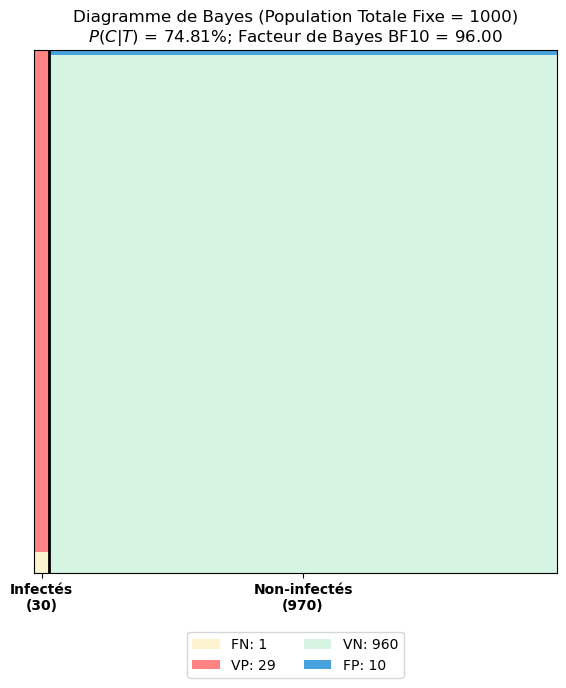
\includegraphics[width=0.5\linewidth]{Images/diagramme_bayes_crise}
		\label{fig:diagramme_bayes_crise}
	\end{figure}
\end{frame}

\begin{frame}{Low-Activity Period}
	During a low-activity period, suppose we obtain a positive test result. What is the probability of having Covid-19 given a positive test?
	\begin{itemize}
		\item The prior probability of having Covid-19: $P(C) = 0.001$. 
		\item The test sensitivity is 96\%, so: $P(T \mid C) = 0.96$.
		\item The test specificity is 99\%, so: $P(\bar{T} \mid \bar{C}) = 0.99$.
	\end{itemize}
	\vspace{0.5cm}
	\pause
	Let us do a quick sanity check for a group of 1000 people:
	\begin{itemize}
		\item There is 1 infected person, who will likely test positive.
		\pause
		\item There are 999 non-infected people. Since there is a 1\% chance of a false positive, this results in about 10 false positives.
		\pause
		\item Therefore, there are roughly 11 people with a positive test, and 10 of them are not infected. This means a person with a positive test has approximately a 9\% chance of being infected.
	\end{itemize}
\end{frame}

\begin{frame}{Low-Activity Period - Calculation}
	The marginal probability is:
	\begin{equation}
		\begin{aligned}
			P(T) &= P(T \cap C) + P(T \cap \bar{C}) \\
			&= P(T \mid C) P(C) + P(T \mid \bar{C}) P(\bar{C}) \\
			&= P(T \mid C) P(C) + (1 - P(\bar{T} \mid \bar{C})) (1 - P(C)) \\
			&= 0.96 \times 0.001 + (1 - 0.99) \times (1 - 0.001) \\
			&= 0.00096 + 0.00999 = 0.01095
		\end{aligned}
		\nonumber
	\end{equation}
	\pause
	We can now compute the posterior probability:
	\begin{equation}
		\begin{aligned}
			P(C \mid T) &= \frac{P(T \mid C) P(C)}{P(T)} \\
			&= \frac{0.96 \times 0.001}{0.01095} 
			= \frac{0.00096}{0.01095} \\
			&\approx 0.088
		\end{aligned}
		\nonumber
	\end{equation}
\end{frame}

\begin{frame}{Low-Activity Period - Visualization}
	\begin{figure}
		\centering
		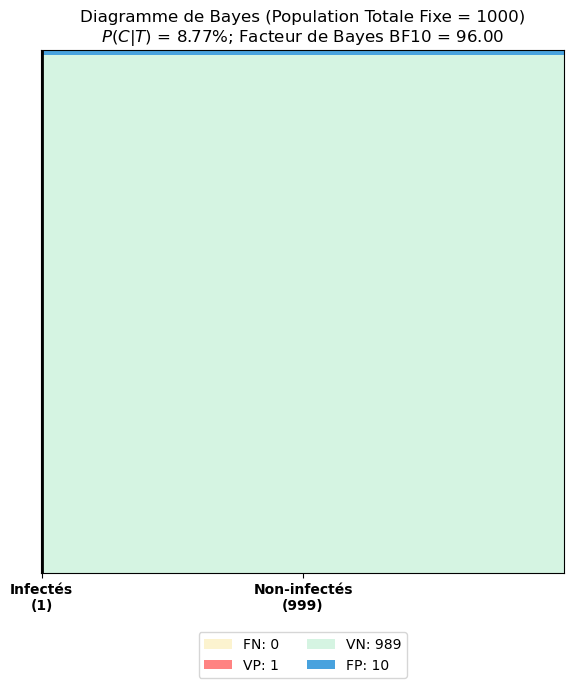
\includegraphics[width=0.5\linewidth]{Images/diagramme_bayes_accalmie}
		\label{fig:diagramme_bayes_accalmie}
	\end{figure}
\end{frame}


\begin{frame}{Low-Activity Period with a Second Positive Test}
	During a low-activity period, suppose we obtain a \textbf{second} positive test result. We assume this test is conditionally independent of the first one given the disease status. What is the probability of having Covid-19 given this second positive test?
	\begin{itemize}
		\item The prior probability of having Covid-19: $P(C) = 0.088$. This is the updated probability of having Covid-19 after the first positive test.
		\item The test sensitivity is 96\%, so: $P(T \mid C) = 0.96$.
		\item The test specificity is 99\%, so: $P(\bar{T} \mid \bar{C}) = 0.99$.
	\end{itemize}
\end{frame}

\begin{frame}{Low-Activity Period with a Second Positive Test - Calculation}
	The marginal probability is:
	\begin{equation}
		\begin{aligned}
			P(T) &= P(T \cap C) + P(T \cap \bar{C}) \\
			&= P(T \mid C) P(C) + P(T \mid \bar{C}) P(\bar{C}) \\
			&= P(T \mid C) P(C) + (1 - P(\bar{T} \mid \bar{C})) (1 - P(C)) \\
			&= 0.96 \times 0.088 + (1 - 0.99) \times (1 - 0.088) \\
			&= 0.08448 + 0.00912 = 0.0936
		\end{aligned}
		\nonumber
	\end{equation}
	\pause
	We can now compute the posterior probability:
	\begin{equation}
		\begin{aligned}
			P(C \mid T) &= \frac{P(T \mid C) P(C)}{P(T)} \\
			&= \frac{0.96 \times 0.088}{0.0936} 
			= \frac{0.08448}{0.0936} \\
			&\approx 0.903
		\end{aligned}
		\nonumber
	\end{equation}
\end{frame}

\subsection{Bayes Factor}

\begin{frame}{Introducing an Alternative Form}
	We have seen that Bayes' theorem for two events $A$ and $B$ is written as:
	\begin{equation}
		P(A \mid B) = \frac{P(B \mid A) P(A)}{P(B)}
		\nonumber
	\end{equation}
	\pause
	In a similar manner, we can write:
	\begin{equation}
		P(\bar{A} \mid B) = \frac{P(B \mid \bar{A}) P(\bar{A})}{P(B)}
		\nonumber
	\end{equation}
	\pause
	Dividing these two equations yields:
	\begin{equation}
		\frac{P(A \mid B)}{P(\bar{A} \mid B)} = \frac{\frac{P(B \mid A) P(A)}{P(B)}}{\frac{P(B \mid \bar{A}) P(\bar{A})}{P(B)}}
		\nonumber
	\end{equation}	
\end{frame}

\begin{frame}{Bayes Factor}
	The previous expression simplifies to:
	\begin{equation}
		\frac{P(A \mid B)}{P(\bar{A} \mid B)} = \frac{P(B \mid A)}{P(B \mid \bar{A})} \frac{P(A)}{P(\bar{A})}
		\nonumber
	\end{equation}
	\begin{block}{Definition: Bayes Factor}
		Given two events $A$ and $B$, the Bayes Factor is defined by:
		\begin{equation}
			\begin{cases}
				\text{BF}_{10}(B) = \displaystyle \frac{P(B \mid A)}{P(B \mid \bar{A})} \\[10pt]
				\text{BF}_{10}(\bar{B}) = \displaystyle \frac{P(\bar{B} \mid A)}{P(\bar{B} \mid \bar{A})}
			\end{cases}
			\nonumber
		\end{equation}
	\end{block}
	Note: The subscript $10$ denotes that condition $A$ is true in the numerator and false in the denominator. We could just as easily define a Bayes Factor $\text{BF}_{01}$.
\end{frame}

\begin{frame}{Alternative Form of Bayes' Theorem}
	Using the Bayes Factor, we obtain an alternative formulation of Bayes' theorem using odds:
	\begin{equation}
		\odds(A \mid B) = \text{BF}_{10}(B) \, \odds(A)
		\nonumber
	\end{equation}
	\pause
	We can apply this formulation to our Covid-19 problem. With a sensitivity of 96\% and a specificity of 99\%, we can compute the Bayes Factor:
	\begin{equation}
		\begin{aligned}
			\text{BF}_{10}(T) &= \frac{P(T \mid C)}{P(T \mid \bar{C})} \\
			&= \frac{P(T \mid C)}{1 - P(\bar{T} \mid \bar{C})} \\
			&= \frac{0.96}{1 - 0.99} \\
			&= 96
		\end{aligned}
		\nonumber
	\end{equation}
\end{frame}

\begin{frame}{Alternative Form of Bayes' Theorem}
	We can use this Bayes Factor to efficiently solve the previous problems. We simply need to compute the odds associated with the prior probability. Recall that:
	\begin{equation}
		\odds = \frac{p}{1 - p} \Longleftrightarrow p = \frac{\odds}{\odds + 1}
		\nonumber
	\end{equation}
	\begin{itemize}
		\item If the prior probability is 3\%, the odds are $3:97$, and thus the posterior odds are $288:97$. This yields a posterior probability of 0.748.
		\item If the prior probability is 0.1\%, the odds are $1:999$, and thus the posterior odds are $96:999$. This yields a posterior probability of 0.088.
		\item If the prior probability is 8.8\%, the odds are $11:114$, and thus the posterior odds are $1056:114$. This yields a posterior probability of 0.093.
	\end{itemize}
\end{frame}

\subsection{Recursive Nature of Bayes' Theorem}

\begin{frame}{Movie Reviews}
	A new movie has just been released in theaters. We represent our opinion by a random variable $A$ which takes the value 0 if we have a negative view of the movie and 1 otherwise. Having no specific prior opinion, we represent our \textbf{prior} belief with the following probability mass function:
	\begin{equation}
		\begin{cases}
			P(A = 0) = 0.5 \\
			P(A = 1) = 0.5
		\end{cases}
		\nonumber
	\end{equation}
	\pause
	We then read a series of reviews $C$, assumed to be conditionally independent given $A$, which can be either negative ($C=0$) or positive ($C=1$). We also define a sensitivity and specificity:
	\begin{itemize}
		\item \textbf{Sensitivity}: Probability that a review is positive for a movie we like: 0.65
		\item \textbf{Specificity}: Probability that a review is negative for a movie we dislike: 0.75
	\end{itemize}
\end{frame}

\begin{frame}{Movie Reviews - Visualization}
	\begin{columns}
		\begin{column}{0.45\textwidth}
			After reading 2 negative reviews and 2 positive reviews, we now hold a slightly favorable view of the movie. To achieve this result, we sequentially applied Bayes' theorem 4 consecutive times, using the posterior probability of the previous step as the prior probability for the current step:
		\end{column}
		\begin{column}{0.55\textwidth}
			\begin{figure}
				\centering
				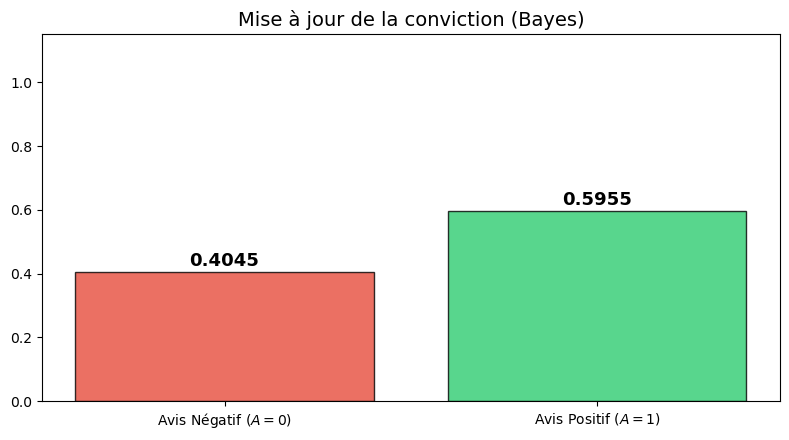
\includegraphics[width=1.0\linewidth]{Images/bayes_recursif}
				\label{fig:bayes_recursive}
			\end{figure}
		\end{column}		
	\end{columns}
	\vspace{0.5cm}
	Note: Using the Bayes Factors $\text{BF}_{10}(C=1)$ and $\text{BF}_{10}(C=0)$ makes this problem very fast to solve:
	\begin{equation}
		\odds_{\text{final}} = \text{BF}_{10}(C=0)^2 \, \text{BF}_{10}(C=1)^2 \, \odds_{\text{initial}}
		\nonumber
	\end{equation}
\end{frame}

\subsection{Conclusion}

\begin{frame}{The Essence of Bayesian Reasoning}
	Bayesian inference is not merely a formula; it is a \textbf{framework for updating knowledge}.
	\vspace{0.3cm}
	\begin{itemize}
		\item \textbf{The weight of the context}: The \textit{posterior} probability depends just as much on the strength of the evidence (likelihood) as it does on what was known before (prior). 
		\begin{itemize}
			\item[$\rightarrow$] \textit{An excellent test evaluated on a rare disease primarily yields false positives.}
		\end{itemize}
		\pause
		\item \textbf{The Bayes Factor ($\text{BF}_{10}$)}: This is the conviction multiplier. It measures the intrinsic strength of a piece of data, completely independent of the baseline context.
		\pause
		\item \textbf{The recursive nature}: Today's \textit{posterior} becomes tomorrow's \textit{prior}. This is the core principle of continuous learning.
	\end{itemize}
\end{frame}